\section{Datasets and analysis}

Various benchmark datasets have been proposed to train and evaluate
definition models. Table \ref{tab:datasets} lists datasets applied in different definition modeling methods. In this section, we provide brief descriptions of each
dataset and provide an analysis of various characteristics of the datasets.

\begin{table}[h]
    \centering
    \caption{Datasets used in definition modeling.}
    \begin{tabular}{|ll|}
        \hline
        Dataset          & Methods                              \\
        \hline
        Oxford           & \cite{bevilacqua_generationary_2020,
            chang_what_2019,
            gadetsky_conditional_2018,
            ishiwatari_learning_2019,
            li_explicit_2020,
            mickus_mark_2019,
            reid_vcdm_2020,
            washio_bridging_2019}                               \\
        WordNet          & \cite{bevilacqua_generationary_2020,
            ishiwatari_learning_2019,
            kabiri_evaluating_2020,
            li_explicit_2020,
            mickus_mark_2019,
            noraset_definition_2016,
            washio_bridging_2019}                               \\
        Urban Dictionary & \cite{reid_vcdm_2020,
            ishiwatari_learning_2019,
            ni_learning_2017}                                   \\
        Wikipedia        & \cite{huang_cdm_2021,
            reid_vcdm_2020}                                     \\
        Wiktionary       & \cite{bevilacqua_generationary_2020,
            kabiri_evaluating_2020}                             \\
        OmegaWiki        & \cite{kabiri_evaluating_2020}        \\
        Hei++            & \cite{bevilacqua_generationary_2020} \\
        \hline
    \end{tabular}
    \label{tab:datasets}
\end{table}

\noindent\textbf{Oxford Dictionary:}
\textit{The Oxford Dictionary of
    English}\footnote{\href{https://languages.oup.com/}{https://languages.oup.com/}}
is a free dictionary of English words and phrases. Collected by Gadetsky et
al. \cite{gadetsky_conditional_2018}, this dataset features contextual information for each word along with
the definition. This dataset is useful for
evaluating the ability of a model to generate definitions for polysemous
words.

\noindent\textbf{GCIDE/WordNet:}
\textit{The GNU Collaborative International Dictionary of
    English}\footnote{\href{https://gcide.gnu.org.ua/}{https://gcide.gnu.org.ua/}}
(GCIDE) is a free dictionary supplemented with some definitions from
WordNet\footnote{\href{https://wordnet.princeton.edu/}{https://wordnet.princeton.edu/}}.
GCIDE is a useful corpus for
dictionary definitions for general words. This dataset was modified by
Noraset et al. \cite{noraset_definition_2016} for their original definition
model. Kabiri et al. \cite{kabiri_evaluating_2020} also provide a modified
dataset for their method.

\noindent\textbf{Urban Dictionary:}
\textit{The Urban
    Dictionary}\footnote{\href{https://www.urbandictionary.com/}{https://www.urbandictionary.com/}}
is a free dictionary of slang words and phrases where definitions are
crowd-sourced by users. Proposed by Ni et al. \cite{ni_learning_2017}, the
Urban Dictionary dataset is useful for idioms and rarely-used phrases which
are not contained in other dictionary datasets due to only containing slang
definitions.

\noindent\textbf{Wikipedia:}
\textit{The English
    Wikipedia}\footnote{\href{https://en.wikipedia.org/}{https://en.wikipedia.org/}}
is a free online encyclopedia. Collected by Ishiwatari et al.
\cite{ishiwatari_learning_2019}, it combines the useful tasks of WordNet,
Oxford Dictionary, and Urban Dictionary, since it contains descriptions of
many concepts along with context to be used in context-aware models.

\noindent\textbf{Wiktionary:}
\textit{Wiktionary}\footnote{\href{https://en.wiktionary.org/}{https://en.wiktionary.org/}}
is a free online dictionary from the same parent organization as Wikipedia
(Wikimedia Foundation). It is useful as it provides a definitions for a large
number of languages which can allow for multi-lingual definition modeling. We
share statistics for the English version of Wiktionary, since most definition
modeling methods focus on English.

\noindent\textbf{OmegaWiki:}
Similar to Wiktionary, \textit{OmegaWiki} is a multi-lingual dictionary. The
goal of OmegaWiki is to create a lexical resource with all definitions of all
words in every language. Kabiri et al. \cite{kabiri_evaluating_2020} use this
resource due to the availability of a variety of languages.

\noindent\textbf{Hei++:}
\textit{Hei++}\footnote{\href{http://generationary.org/}{http://generationary.org/}}
is a unique evaluation dataset proposed by Bevilacqua et al.
\cite{bevilacqua_generationary_2020}. Rather than contain singular words or
phrases to define as the other dictionary-based resources, this dataset is comprised of adjective-noun phrases. An example phrase, \textit{starry sky}, can
be defined as 'The sky as it appears at night, especially when lit by stars.' This is a hand-made dataset created with an expert lexicographer's assistance. As a result, this dataset is small and should be used in model
evaluation rather than training. Our dataset analysis shows no overlap of this
dataset with the other benchmark datasets, implying this dataset can also be
used to evaluate the ability of a model to generalize on never-before-seen
data.

\subsection{Definition statistics}

In our analysis of the datasets above, to distinguish the benchmark datasets
provided by the correlating authors, we use the notations listed in Table
\ref{tab:ds_notations}.

\begin{table}[h]
    \centering
    \caption{Dataset notations.}
    \begin{tabular}{|l|l|}
    \hline
    Dataset                  & Description                                                                                     \\
    \hline
    \textit{wordnet-nor}     & WordNet dataset, from Noraset et al. \cite{noraset_definition_2016}                             \\
    \textit{urban-ni}        & Urban Dictionary dataset, from Ni et al. \cite{ni_learning_2017}                                \\
    \textit{oxford-gad}      & The Oxford Dictionary of English dataset, from Gadetsky et al. \cite{gadetsky_conditional_2018} \\
    \textit{wordnet-ish}     & WordNet dataset, from Ishiwatari et al. \cite{ishiwatari_learning_2019}                         \\
    \textit{wikipedia-ish}   & Wikipedia dataset, from Ishiwatari et al. \cite{ishiwatari_learning_2019}                       \\
    \textit{wikitionary-kab} & Wikitonary English dataset, from Kabiri et al. \cite{kabiri_evaluating_2020}                    \\
    \textit{wordnet-kab}     & WordNet dataset, from Kabiri et al. \cite{kabiri_evaluating_2020}                               \\
    \textit{omega-kab}       & OmegaWiki dataset, from Kabiri et al. \cite{kabiri_evaluating_2020}                             \\
    \textit{hei++-bev}       & Hei++ dataset, from Bevilacqua et al. \cite{bevilacqua_generationary_2020}                      \\
    \hline
\end{tabular}

    \label{tab:ds_notations}
\end{table}

First, in Table \ref{tab:defs}, we provide some analysis of the definition
statistics of the datasets. We evaluate all splits (train, test, and validate)
for each dataset by combining all the words and corresponding definitions. The
table shows the number of unique words and a total number of definitions for each
dataset. Of note, some datasets provide the same definition for the same word,
meant to be used in a context-aware model. In this analysis, we ignore the
context phrases and treat these duplicate definitions as independent. We also
show the mean length of the definitions, the standard deviation of the lengths,
and the definitions per word.


Next, in Table \ref{tab:polys}, we show the number of polysemous words in each
dataset. As with the definition statistics, we treat exact duplicate definitions
independently because they have different contexts. The number of polysemes is
calculated as the number of words or phrases with more than one definition
in the dataset. Finally, we show the ratio of the number of polysemous words to the total
number of words in the dataset as a percentage. It is important to evaluate the polysemous
data due to the difficulty of predicting definitions for polysemous words.

\begin{table}[h]
    \centering
    \caption{Definition statistics.}
    \begin{tabular}{|l|rr|rrr|}
    \hline
    Dataset        & Words   & Definitions & DPW  & Mean length & SD length \\
    \hline
    wikipedia-ish  & 168,753 & 988,690     & 5.86 & 5.99        & 4.53      \\
    urban-ni       & 240,334 & 507,504     & 2.11 & 12.11       & 7.71      \\
    wordnet-nor    & 22,554  & 162,925     & 7.22 & 6.60        & 5.73      \\
    oxford-gad     & 36,767  & 122,319     & 3.33 & 11.07       & 7.01      \\
    wiktionary-kab & 17,000  & 29,426      & 1.73 & 7.65        & 6.92      \\
    wordnet-kab    & 20,000  & 28,814      & 1.44 & 10.96       & 7.28      \\
    omega-kab      & 17,000  & 22,735      & 1.34 & 14.61       & 9.83      \\
    wordnet-ish    & 9,937   & 17,410      & 1.75 & 6.64        & 3.78      \\
    hei++-bev      & 713     & 713         & 1.00 & 9.44        & 2.80      \\
    \hline
\end{tabular}

    \label{tab:defs}
\end{table}

\begin{table}[h]
    \centering
    \caption{Polyseme statistics.}
    \small
\begin{tabular}{|l|rrr|}
    \hline
    Dataset    & Words   & Polysemes & Polysemes (\%) \\
    \hline
    WordNet-A  & 22,554  & 22,171    & 98             \\
    Oxford     & 36,767  & 20,563    & 56             \\
    Wikipedia  & 168,753 & 77,278    & 46             \\
    WordNet-B  & 9,937   & 4,221     & 42             \\
    Urban      & 240,334 & 74,620    & 31             \\
    Wiktionary & 17,000  & 4,634     & 27             \\
    Omega      & 17,000  & 3,412     & 20             \\
    WordNet-C  & 20,000  & 3,649     & 18             \\
    Hei++      & 713     & 0         & 0              \\
    \hline
\end{tabular}

    \label{tab:polys}
\end{table}

% \begin{figure}
%     \centering
%     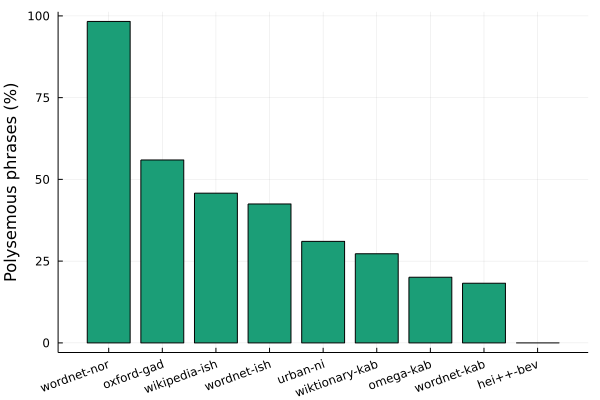
\includegraphics[width=0.65\textwidth]{assets/plots/polys_plot.png}
%     \caption{Plot of polyseme statistics, where the percentage of words or
%         phrases that are polysemous are shown.} \label{fig:polys}
% \end{figure}

Our following analysis is on the overlap present across the benchmark datasets. We
show the number of words in each dataset which are present in all other datasets
as a percentage. This allows us to identify the most similar
and most unique datasets. The overlap of each dataset is calculated as the words
that are present in each other datasets. The overlap of each dataset is
shown in Table \ref{tab:overlap_all}. The values in the table represent the percent of the 
words in the row dataset that are present in the column dataset. For example, $25\%$ of the 
words in the OmegaWiki dataset are present in the Oxford dataset.
We also show the uniqueness of each dataset, calculated as the percentage of words in a dataset that are not present in any other dataset. The plot of dataset uniqueness is shown in Figure \ref{fig:uniqueness_plot}. The uniqueness of the Hei++ dataset is due to two factors: its relatively small size and focuses on adjective-noun phrases.

% \begin{figure}
%     \centering
%     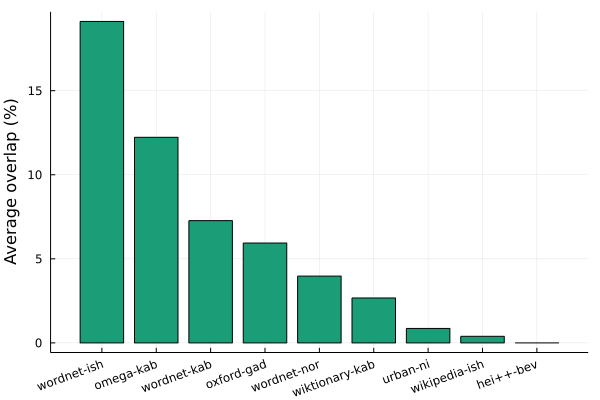
\includegraphics[width=0.55\textwidth]{assets/plots/avg_overlap.png}
%     \caption{Plot of average dataset overlap.}
%     \label{fig:avg_overlap}
% \end{figure}

\begin{figure}
    \centering
    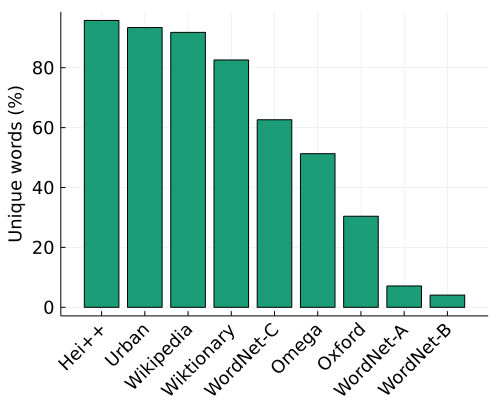
\includegraphics[width=0.45\textwidth]{assets/plots/uniqueness_plot.png}
    \caption{Plot of dataset uniqueness.}
    \label{fig:uniqueness_plot}
\end{figure}

\begin{table}
    \centering
    \caption{Individual dataset overlap.}
    \begin{tabular}{|l|ccccccccc|}
    \hline
    Dataset    & Hei++ & Omega & Oxford & Urban & Wiki & Wiktionary & \makecell{Word\\Net-A} & \makecell{Word\\Net-B} & \makecell{Word\\Net-C} \\
    \hline
    Hei++      & -     & 0\%   & 0\%    & 2\%   & 2\%       & 0\%        & 0\%       & 0\%       & 1\%       \\
    Omega      & 0\%   & -     & 25\%   & 13\%  & 12\%      & 2\%        & 19\%      & 8\%       & 6\%       \\
    Oxford     & 0\%   & 5\%   & -      & 7\%   & 6\%       & 1\%        & 14\%      & 5\%       & 4\%       \\
    Urban      & 0\%   & 1\%   & 2\%    & -     & 1\%       & 0\%        & 1\%       & 1\%       & 0\%       \\
    Wikipedia  & 0\%   & 0\%   & 1\%    & 1\%   & -         & 0\%        & 0\%       & 0\%       & 0\%       \\
    Wiktionary & 0\%   & 1\%   & 5\%    & 4\%   & 2\%       & -          & 3\%       & 1\%       & 1\%       \\
    WordNet-A  & 0\%   & 3\%   & 10\%   & 4\%   & 3\%       & 1\%        & -         & 6\%       & 2\%       \\
    WordNet-B  & 0\%   & 11\%  & 35\%   & 15\%  & 11\%      & 2\%        & 53\%      & -         & 8\%       \\
    WordNet-C  & 0\%   & 5\%   & 16\%   & 7\%   & 7\%       & 1\%        & 11\%      & 5\%       & -         \\
    \hline
\end{tabular}

    \label{tab:overlap_all}
\end{table}

In most of the datasets, some definitions consist only of a single word. Single-word
definitions may cause evaluation criteria such as BLEU to be challenging to
improve. We show the percentage of definitions in each dataset which consists of
only a single word. We also show the number of single-word definitions in each
dataset which are considered to be a synonym of the word or phrase being
defined. We used WordNet synsets to identify synonymous words. The
single word definition analysis is shown in Figure \ref{fig:single_word_defs}.

\begin{figure}
    \centering
    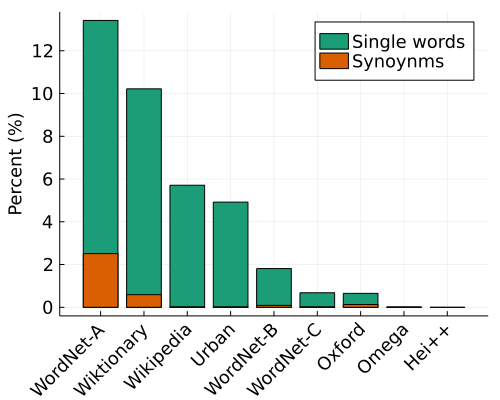
\includegraphics[width=0.45\textwidth]{assets/plots/syn_counts.png}
    \caption{Plot of single word definitions.}
    \label{fig:single_word_defs}
\end{figure}

Across every benchmark dataset, there does not exist a word that is present in each dataset. However, there is a word that exists in $8$ out of $9$ datasets: the word \textbf{movement}. We show selected definitions for this word in Table \ref{tab:movement}. Several different word senses can be seen across the dataset, such as movement as something moving, a specific album, bowel movement, and even the illusion of something moving.

\begin{table}[h]
    \centering
    \caption{Definitions for the word \textbf{movement}.}
    \begin{tabular}{|l|l|}
    \hline
    Dataset        & Definition                                                                                                                                  \\
    \hline
    wordnet-nor    & \makecell[l]{a natural event that involves a change in the position or location of something}                                                             \\
    \hline
    oxford-gad     & \makecell[l]{a group of people with a common ideology who try together to achieve\\ certain general goals}                                                  \\
    \hline
    wordnet-ish    & a major self-contained part of a symphony or sonata                                                                                         \\
    \hline
    wikipedia-ish  & album by new order                                                                                                                          \\
    \hline
    urban-ni       & [pot credit] slang, to hit on a woman                                                                                                       \\
    \hline
    wordnet-kab    & \makecell[l]{an optical illusion of motion produced by viewing a rapid succession of\\ still pictures of a moving object}                                   \\
    \hline
    wiktionary-kab & the deviation of a pitch from ballistic flight                                                                                              \\
    \hline
    omega-kab      & \makecell[l]{what a dogs body releases from time to time as a little pile of waste\\
                    remaining from digestion , after it has been collected in the colon .} \\
    \hline
\end{tabular}

    \label{tab:movement}
\end{table}

